Первый вариант архитектуры компонента Remap, содержащий специальный модуль синхронизации тактовых доменов, представлен на рисунке \ref{fig:remap_cds}.\par
\begin{figure}[ht]
    \centering
    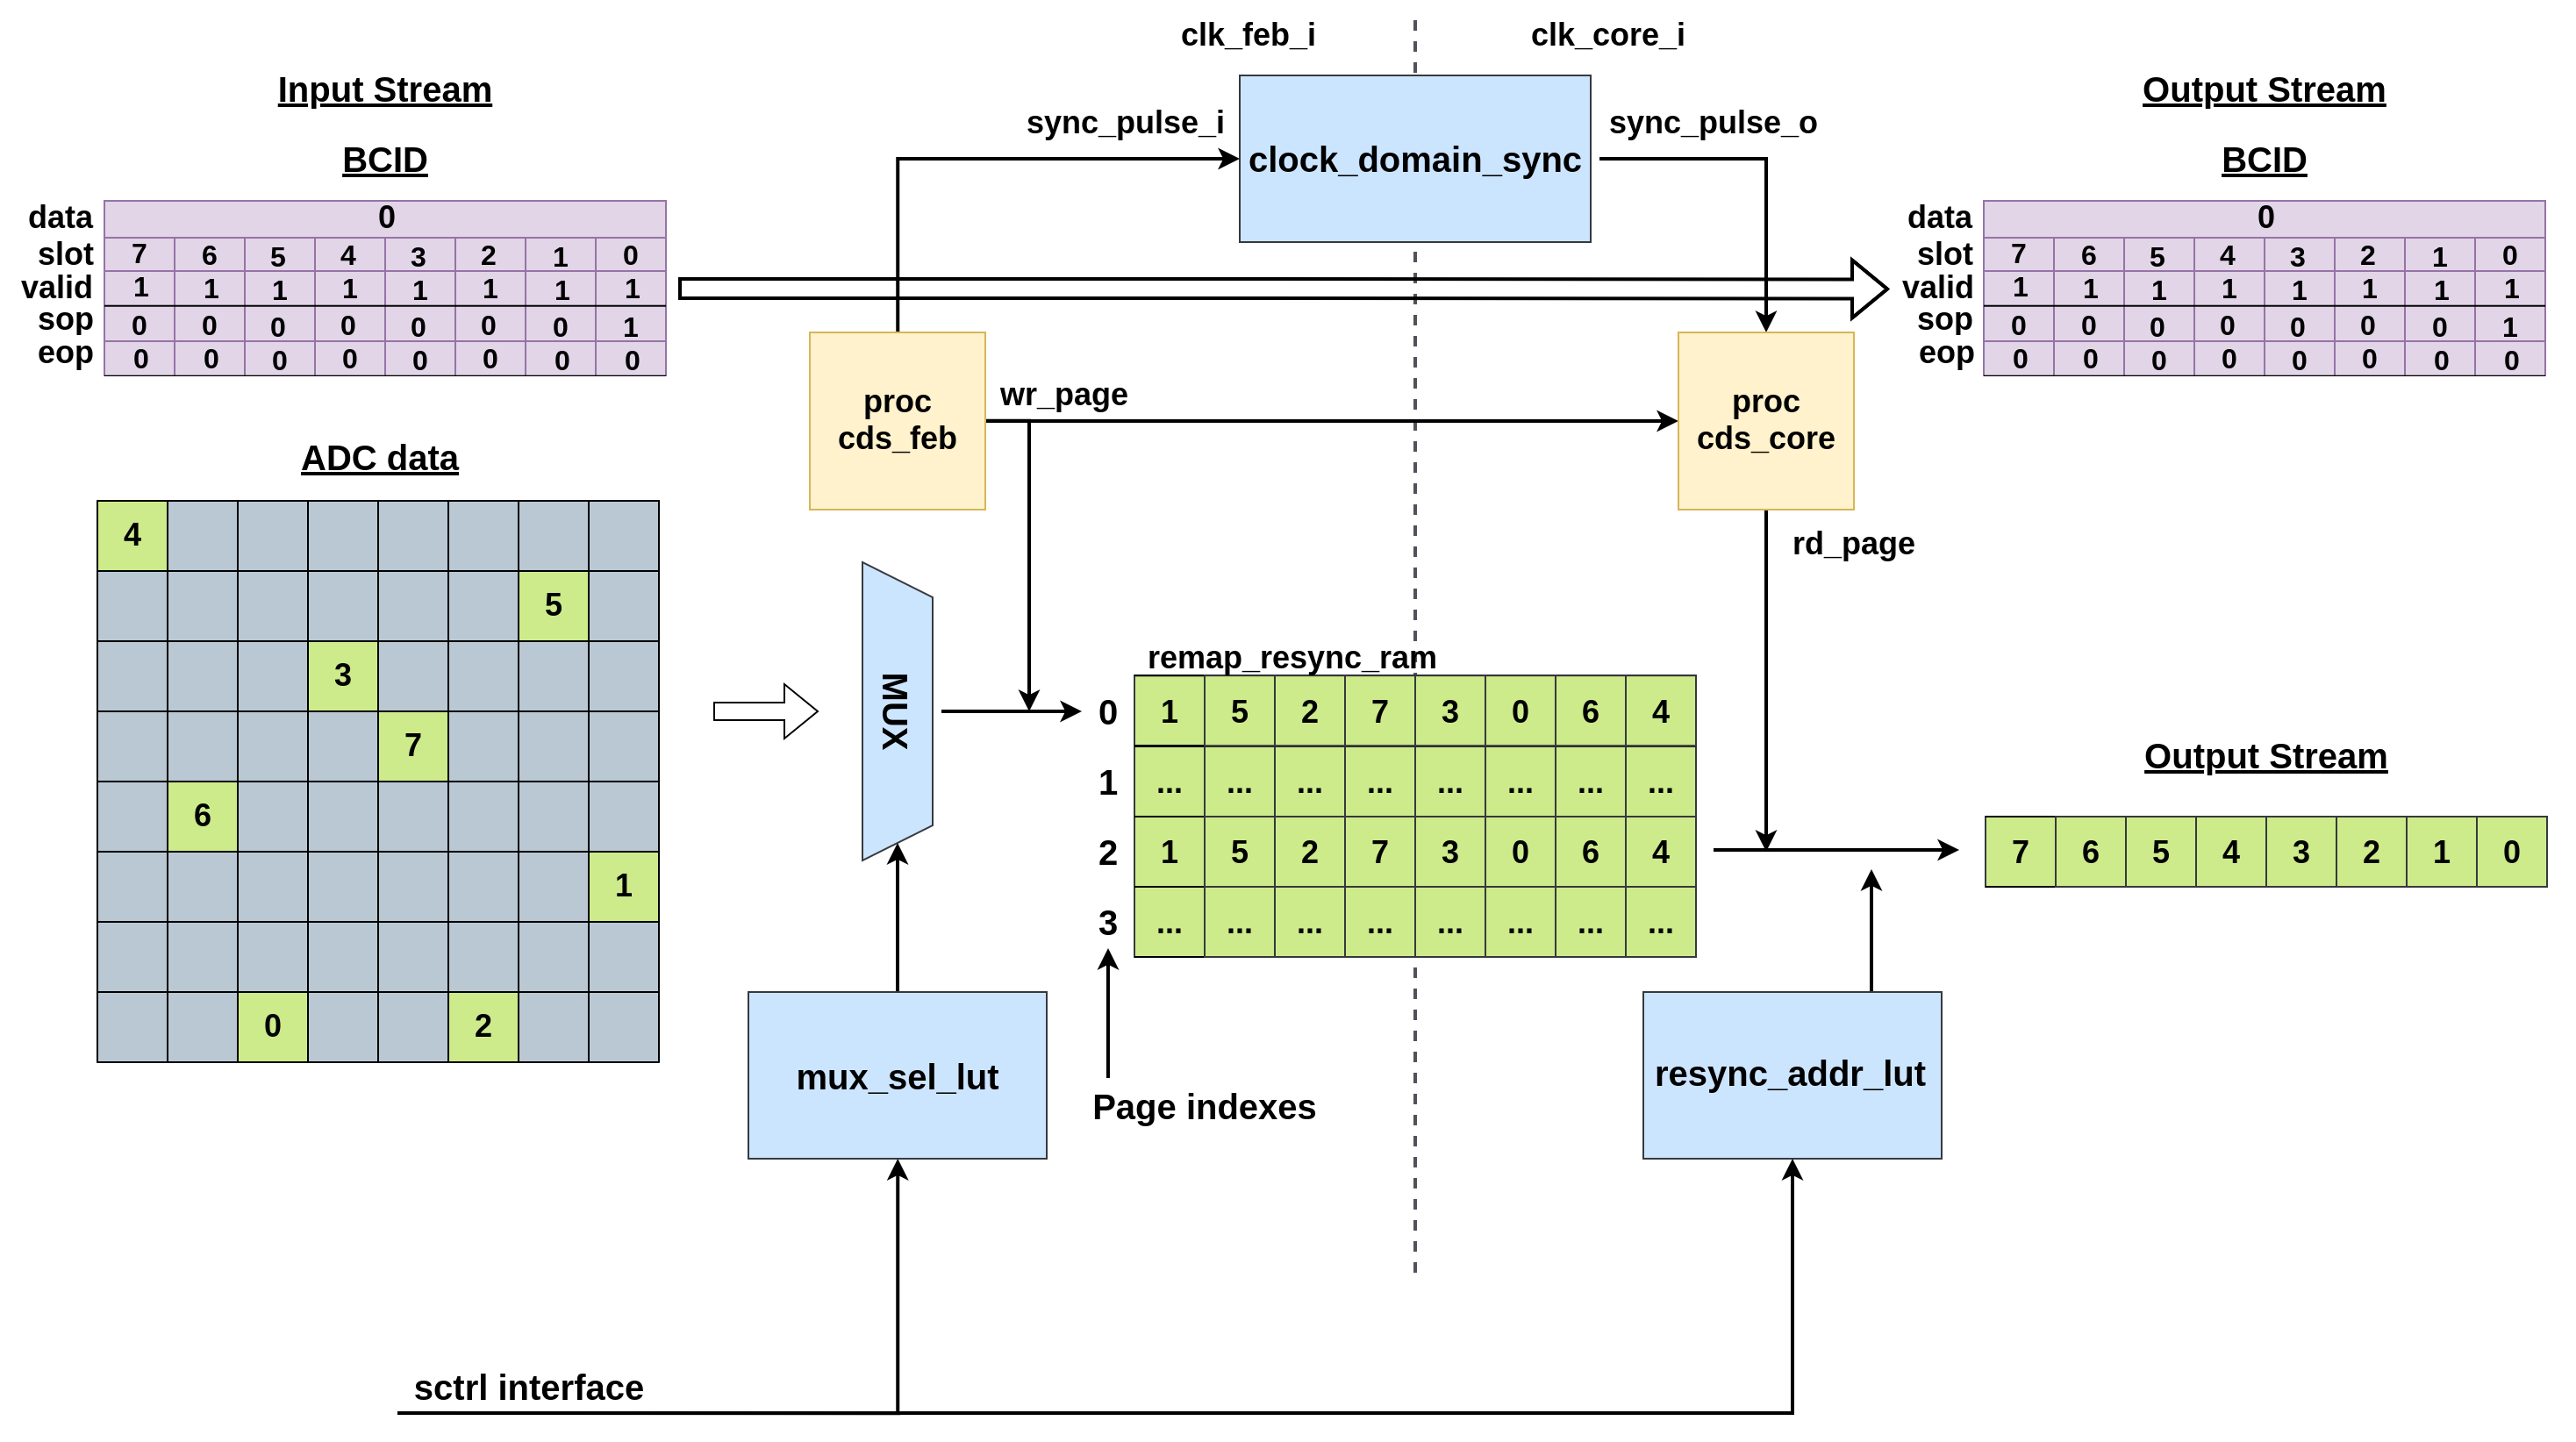
\includegraphics[width=\linewidth]{remap_cds.png}
    \caption{Схема архитектуры модуля Remap с модулем синхронизации тактовых доменов ПЕРЕВЕСТИ}
    \label{fig:remap_cds}
\end{figure}\par
Основной особенностью этой архитектуры является то, что в качестве буфера для мультиплексированных данных используется блок двухпортовой RAM памяти. Эта память разбита на несколько страниц, каждая из которых имеет размер, достаточный для хранения захваченной информации, относящейся к одному столкновению пучков. Чтение данных из страницы начинается лишь только после после её полного заполнения записывающей стороной.\par
